% Detailed model structure for LidarRoofSegNet.
%   Row 1: DGCNN encoder + Conv1d decoder (the embedding network, trainModel.py).
%   Row 2: plane-aware refinement head (cluster graph -> 11-d features -> LightGBM
%          merge classifier -> pairwise-greedy merge).
% Dimensions match trainModel.py: input_dim=6, k=20, emb_dim=128, output_dim=64,
% max_points N=4096. Self-contained standalone TikZ — compiles in Overleaf as-is.
\documentclass[border=6pt]{standalone}
\usepackage{tikz}
\usepackage{amsmath}
\usetikzlibrary{arrows.meta, positioning, fit, backgrounds, calc, shapes.geometric}

\definecolor{cEnc}{HTML}{4C72B0}
\definecolor{cDec}{HTML}{4C9F70}
\definecolor{cContrib}{HTML}{C44E52}
\definecolor{cMisc}{HTML}{6E7B8B}

\begin{document}
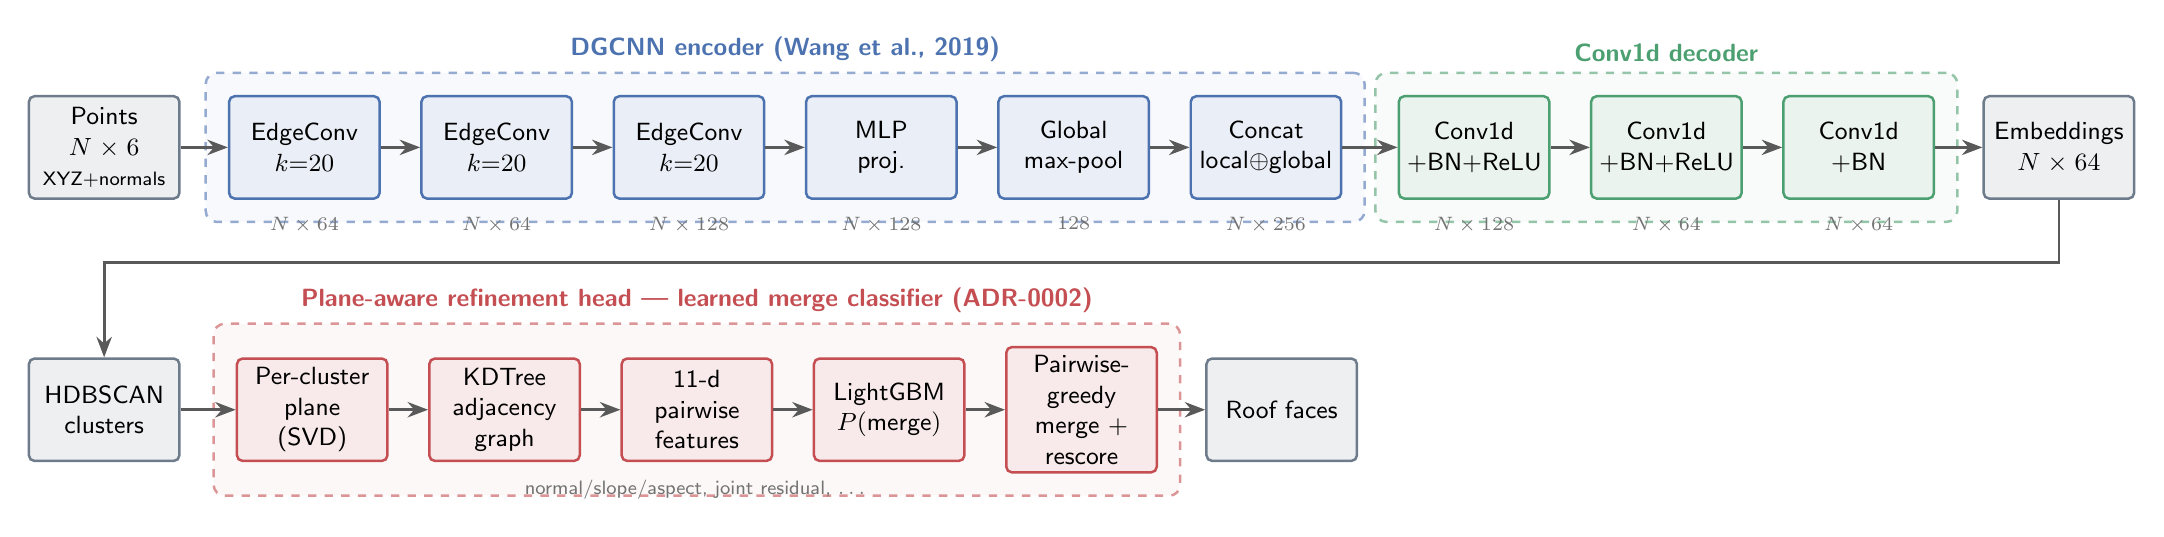
\begin{tikzpicture}[
  font=\sffamily,
  >={Stealth[length=2.6mm]},
  lyr/.style={rectangle, rounded corners=2pt, draw=#1, line width=0.9pt,
              fill=#1!12, align=center, minimum height=13mm, text width=17mm,
              inner sep=3pt, font=\sffamily\small},
  enc/.style={lyr=cEnc}, dec/.style={lyr=cDec},
  ref/.style={lyr=cContrib}, misc/.style={lyr=cMisc},
  dim/.style={font=\sffamily\scriptsize, text=black!55},
  flow/.style={->, line width=1pt, draw=black!65},
  group/.style={draw=#1!60, dashed, rounded corners=4pt, line width=0.9pt,
                fill=#1!4, inner sep=8pt},
  title/.style={font=\sffamily\bfseries\small, text=#1},
]

% =========================== ROW 1 : embedding network ===========================
\node[misc] (in) {Points\\$N\times6$\\\scriptsize XYZ+normals};
\node[enc, right=6mm of in]  (e1) {EdgeConv\\$k{=}20$};
\node[enc, right=5mm of e1]  (e2) {EdgeConv\\$k{=}20$};
\node[enc, right=5mm of e2]  (e3) {EdgeConv\\$k{=}20$};
\node[enc, right=5mm of e3]  (proj){MLP\\proj.};
\node[enc, right=5mm of proj](gpool){Global\\max-pool};
\node[enc, right=5mm of gpool](cat){Concat\\local$\oplus$global};
\node[dec, right=7mm of cat] (d1) {Conv1d\\+BN+ReLU};
\node[dec, right=5mm of d1]  (d2) {Conv1d\\+BN+ReLU};
\node[dec, right=5mm of d2]  (d3) {Conv1d\\+BN};
\node[misc, right=6mm of d3] (emb) {Embeddings\\$N\times64$};

% output-dim annotations under encoder/decoder layers
\node[dim, below=1mm of e1]  {$N\times64$};
\node[dim, below=1mm of e2]  {$N\times64$};
\node[dim, below=1mm of e3]  {$N\times128$};
\node[dim, below=1mm of proj]{$N\times128$};
\node[dim, below=1mm of gpool]{$128$};
\node[dim, below=1mm of cat] {$N\times256$};
\node[dim, below=1mm of d1]  {$N\times128$};
\node[dim, below=1mm of d2]  {$N\times64$};
\node[dim, below=1mm of d3]  {$N\times64$};

\foreach \a/\b in {in/e1, e1/e2, e2/e3, e3/proj, proj/gpool, gpool/cat, cat/d1, d1/d2, d2/d3, d3/emb}
  \draw[flow] (\a) -- (\b);

\begin{scope}[on background layer]
  \node[group=cEnc, fit=(e1)(e2)(e3)(proj)(gpool)(cat)] (encbox) {};
  \node[group=cDec, fit=(d1)(d2)(d3)] (decbox) {};
\end{scope}
\node[title=cEnc, anchor=south] at (encbox.north) {DGCNN encoder (Wang et al., 2019)};
\node[title=cDec, anchor=south] at (decbox.north) {Conv1d decoder};

% =========================== ROW 2 : refinement head ===========================
\node[misc, below=20mm of in] (clu) {HDBSCAN\\clusters};
\node[ref, right=7mm of clu]  (plane){Per-cluster\\plane (SVD)};
\node[ref, right=5mm of plane](adj) {KDTree\\adjacency graph};
\node[ref, right=5mm of adj]  (feat){11-d pairwise\\features};
\node[ref, right=5mm of feat] (lgb) {LightGBM\\$P(\text{merge})$};
\node[ref, right=5mm of lgb]  (grd) {Pairwise-greedy\\merge + rescore};
\node[misc, right=6mm of grd] (faces){Roof faces};

\node[dim, below=1mm of feat] {normal/slope/aspect, joint residual, $\dots$};

\foreach \a/\b in {clu/plane, plane/adj, adj/feat, feat/lgb, lgb/grd, grd/faces}
  \draw[flow] (\a) -- (\b);

\begin{scope}[on background layer]
  \node[group=cContrib, fit=(plane)(adj)(feat)(lgb)(grd)] (refbox) {};
\end{scope}
\node[title=cContrib, anchor=south] at (refbox.north) {Plane-aware refinement head — learned merge classifier (ADR-0002)};

% connect row 1 -> row 2 (embeddings feed clustering)
\draw[flow] (emb.south) -- ++(0,-8mm) -| (clu.north);

\end{tikzpicture}
\end{document}
